\documentclass[a4paper,10pt]{article}
%\documentclass[a4paper,10pt]{scrartcl}

\usepackage[utf8x]{inputenc}

\title{Some notes}
\author{Simon}

\pdfinfo{%
  /Title    ()
  /Author   ()
  /Creator  ()
  /Producer ()
  /Subject  ()
  /Keywords ()
}
\usepackage{graphicx}
\begin{document}
\maketitle

\section{Notes opportunistes behavior (20110528)}

Here agents use the fact that when they are waked up after a "waiting time" they are filled up with new "free" energy.

So they move with this "free energy" by bunches of 2, 3 or 4 agents.

The space beetwen bunches should be long enough to allow agents to encounter each other after the "real died" state (waiting but not receveing genomes)

here the "real died" mode is 2.5 time the generations time which is 600 iterations so the dead time is 15000 iterations. It looks very long but bunches sometimes mades very littltes "jump" (in fact 400 units max du two refuel size) and are divided in lot of little groups. And they need in fact to wait only that less than 4 groups  pass near a dead group. The 4th will woke up the over wich in turn will go 4 groups after wake up an other bunch. 
other param :
\begin{itemize}
 \item gEnergyMax : 600
 \item gIteration : 600
 \item gRevive : 400
 \item gSunChan : 2
\end{itemize}


On figure \ref{fig:opportunistsA} we observe two kinds of behavior :
\begin{enumerate}
 \item Red path : Agents go to the orange sun in a spiral and synchronized way by bunches of agents. When reached the sun they don't take any ressource, its jsutto
 \item Green path : Classical "follow the wall" : agents follow the wall by bunches.
\end{enumerate}

\begin{figure}
\begin{center}
\label{fig:opportunistsA}
\caption{Differents kind of oportunists behaviors}
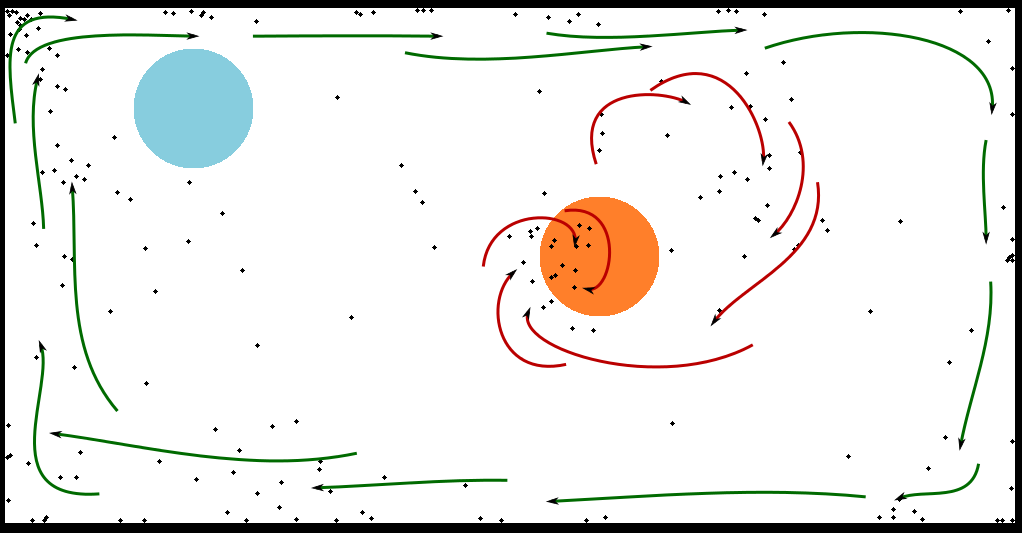
\includegraphics[height=5cm]{201129_agentOportunistes_passlifetorchbis}
\end{center}
\end{figure}

To obtain thoses behavior it was done using a quiet hard "reward" (soon renamed) function with tanh and a n of .7. Because tanh((x-0,7)*alpha) allow a few number of agent to find the right $g_skill$ 
gene we used here 200 agents. diffucltie of the environment is one of the reasons which allow such oportunistic behaviors to emerge.

\subsection{equilibrium}


To find equilibrium in that kind of environment is really hard when astarting like that. Agents look like "locked" on the over side of the genotype. We can see the time taken by mEDEA in figure  \ref{fig:hardtofind} to find a good solution. It's not really clear in that figure because simulation has been stopped to quick but when the good solution is find number of alive agent raise. solution in 

\begin{figure}
	\caption{run where agents stay trapped during a really long time in a poor solution (a few agents alive by cycles). 
		\small a reminder : colors on the plot denote the X position of agents when the take the gene. The more on the left, the more red it will be}
	\begin{center}
 
		\label{fig:hardtofind}
		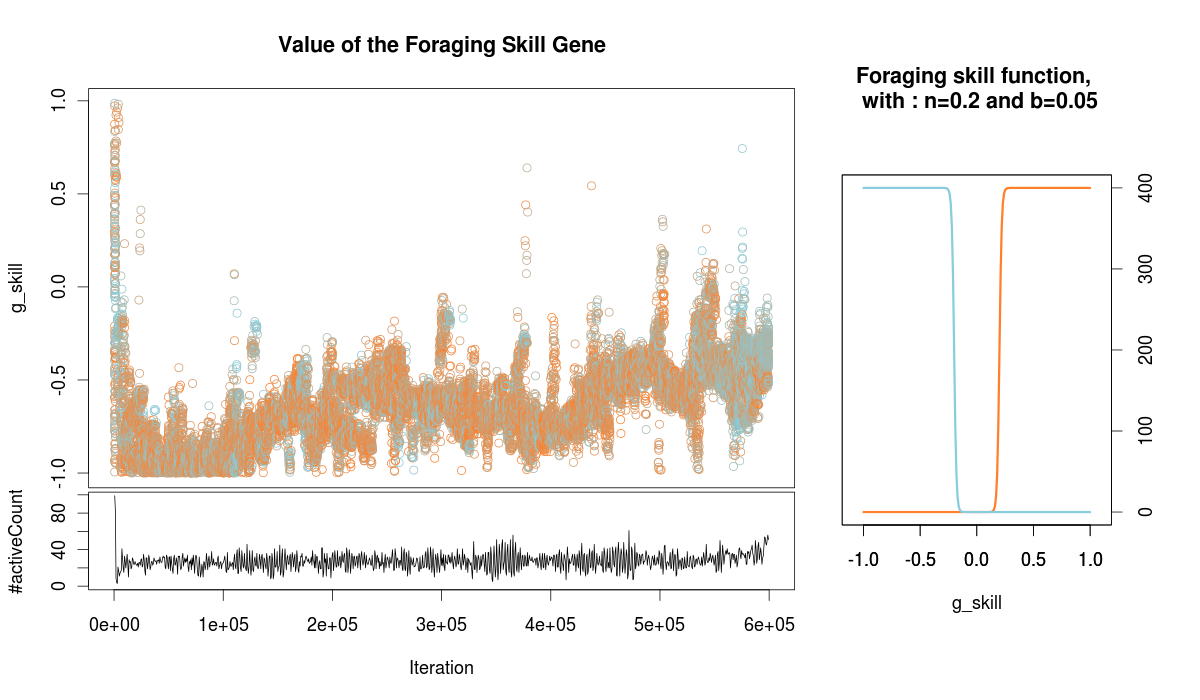
\includegraphics[height=10cm]{tanh_opportunists1}
	\end{center}
\end{figure}

Sometimes even the worst can happend and the flip be done in the wrong side (see Figure \ref{fig:wrongflip})... 

So build environment in order to exclude those case : the solution should be more easy to find quickly : lots of energy points?

%%%%%%%%%%%%%%%%%%%%%%%%%%%%%%%%%%%%%%%%%%%%%%%%%%%%%%%%%%%%%%%%%%%%%%%%%%%%%%%%%%%%%%%%%%%%%%%%%%%%
\begin{figure}
\caption{Aïe! One hope is that maybe we don't wait enough time} 

\begin{center}

\label{fig:wrongflip}
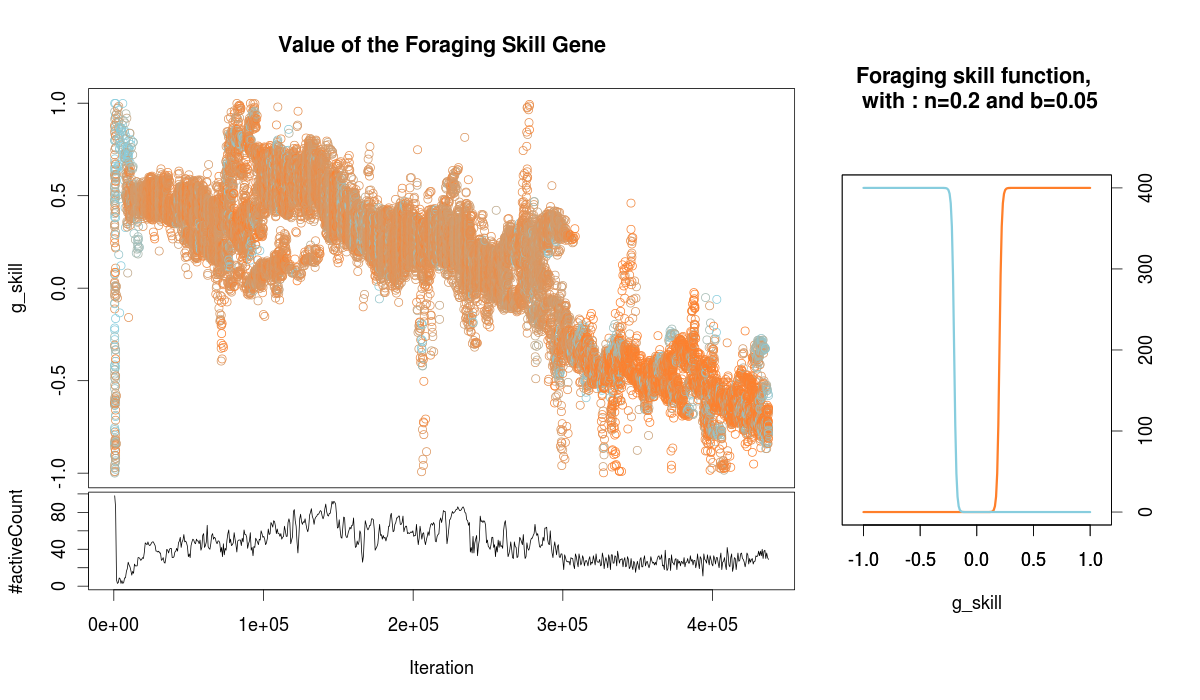
\includegraphics[height=10cm]{tanh_wrongflip}
\end{center}

\end{figure}



%%%%%%%%%%%%%%%%%%%%%%%%%%%%%%%%%%%%%%%%%%%%%%%%%%%%%%%%%%%%%%%%%%%%%%%%%%%%%%%%%%%%%%%%%%%%%%%%%%%%
\begin{figure}
	\caption{Even here not sure that an equilibrium is finded} 

	\begin{center}

	\label{fig:moyen}
	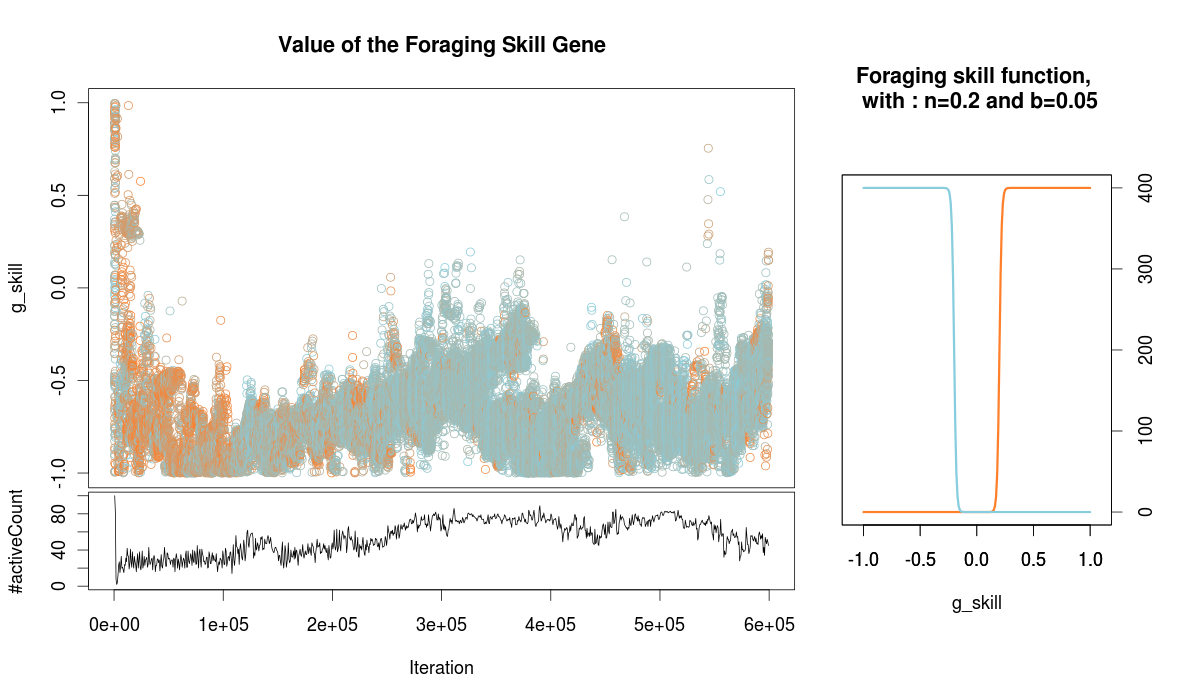
\includegraphics[height=10cm]{tanh_moyenp1}
	\end{center}

\end{figure}

%%%%%%%%%%%%%%%%%%%%%%%%%%%%%%%%%%%%%%%%%%%%%%%%%%%%%%%%%%%%%%%%%%%%%%%%%%%%%%%%%%%%%%%%%%%%%%%%%%%%
\begin{figure}

	\caption{ evaluation 400, revive 400, \emph{max : 1000} !} 
	\begin{center}
		\label{fig:quick}
		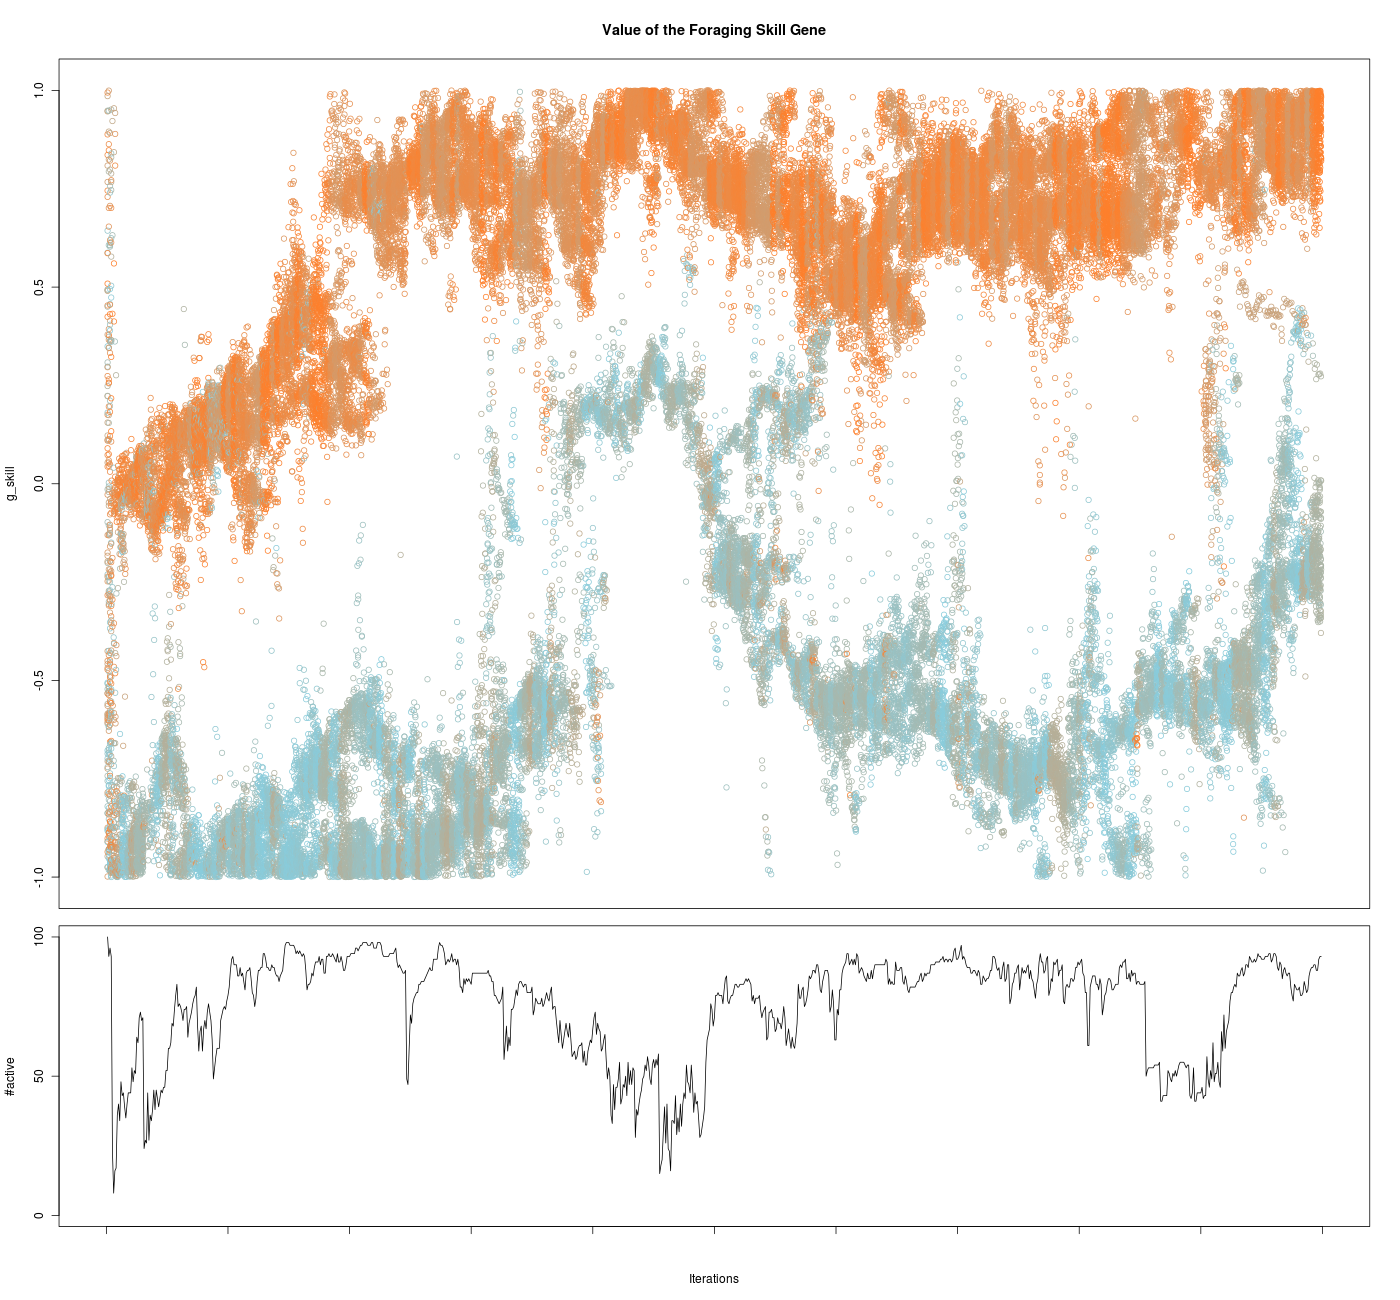
\includegraphics[height=10cm]{tanh_findQuickly}
	\end{center}

\end{figure}

\end{document}
